\documentclass[letterpaper, 12]{article}

%% Language and font encodings
\usepackage[english]{babel}
\usepackage[utf8x]{inputenc}
\usepackage[T1]{fontenc}

%% Sets page size and margins
\usepackage[letterpaper,top=2.5cm,bottom=2cm,left=2cm,right=2cm,marginparwidth=1.75cm]{geometry}

%% Useful packages
\usepackage{amsmath}
\usepackage{amssymb}
\usepackage{amsfonts}
\usepackage{graphicx}
\usepackage{physics}
\usepackage{bbold}
\usepackage[colorinlistoftodos]{todonotes}
\usepackage[colorlinks=true, allcolors=blue]{hyperref}
\usepackage{listings}
\usepackage{multicol}
\usepackage{float}
\usepackage{enumitem}

\usepackage{bm}
\date{\today}

\title{CSC411 Assignment 2}
\author{Yue Guo}
\begin{document}
\maketitle

%\centering
%  \includegraphics[width=0.5\textwidth]{1.3.2/1_3_2_k50.png}
%  \caption{k-NN Regression of $x \in [0, 11]$ with $k$ = 50.}
%\end{figure}

\section{Gaussian}

\subsection{P(y)}

\begin{equation*}
\begin{split}
P( \bm{x} | \mu ,  \sigma) &= \sum_{k = 1}^{K}  P( \bm{x} | y = k, \ mu ,  \sigma) P(y = k | \mu, \sigma) \\
&=  \sum_{k = 1}^{K} \alpha_{k} P( \bm{x} | y = k, \mu ,  \sigma) \\
&= \sum_{k = 1}^{K} \alpha_{k} (\prod_{i=1}^{D} 2\pi \sigma_{i})^{\frac{1}{2}} exp\{{- \sum_{i=1}^{D}} \frac{1}{2 \sigma_{i} ^2} (x_{i} - \mu_{ki})^2 \} 
\end{split}
\end{equation*}
 
\begin{equation*}
\begin{split}
P(y | \bm{x} , \ mu ,  \sigma) &= \frac{P( \bm{x}, y = k | \mu ,  \sigma)}{P( \bm{x} |  \mu ,  \sigma)}
\\
&= \frac{P( \bm{x} | y = k, \ mu ,  \sigma) P(y = k | \mu ,  \sigma)}{P( \bm{x} |  \mu ,  \sigma)}
\\
&=\frac{ \alpha_{k} (\prod_{i=1}^{D} 2\pi \sigma_{i} ^{2})^{-\frac{1}{2}}  exp\{{- \sum_{i=1}^{D}} \frac{1}
{2 \sigma_{i} ^2} (x_{i} - \mu_{ki})^2 \}  }{\sum_{k=1}^{K} \alpha_{k} (\prod_{i=1}^{D} 2\pi \sigma_{i} ^{2})^{-\frac{1}{2}}  exp\{{- \sum_{i=1}^{D}} \frac{1}
{2 \sigma_{i} ^2} (x_{i} - \mu_{ki})^2 \}} \\
\end{split}
\end{equation*}


\subsection{log likelihood}
\begin{equation*}
\begin{split}
-log P(y^{(1)}, x^{(1)}, ..., y^{(N)}, x^{(N)} | \theta) 
&=-log P(y^{(1)}, x^{(1)} | \theta) -log P(y^{(2)}, x^{(2)} | \theta) ... - log( y^{(N)}, x^{(N)} | \theta)\\
&= \sum_{j=1}^{N} -log P(y^{(j)}, x^{(j)} | \theta)\\
&\text{N.B.: in this case, j is the index of the whole data set,} \\
&\text{where as y(j) corresponds to the class that this sample}\\
&\text{ belongs to, and y(i) = k , k in (0, 9)}\\
&= \sum_{j = 1}^{N} -log [\alpha^{y{(j)}} (\prod_{i = 1}^{D} 2 \pi (\sigma_{j} ^{y(i)}) ^2)^{ -\frac{1}{2}}
	 exp\{ - \sum_{i = 1}^{D} \frac{1}{(2 \sigma_{i}^{y(j)}) ^2} (x_{i}^{(j)} - \mu_{i}^{y(j)})^2  \}] \\
&= \sum_{j=1}^{N} \sum_{i = 1}^{D} \frac{1}{2 (\sigma_{i}^{y(j)}) ^2}(x_{i}^{(j)} - \mu_{i}^{y(j)})^2 
	+ \sum_{j = 1}^{N} -log [\alpha^{y(j)} (\prod_{i = 1}^{D} 2 \pi (\sigma_{i}^{y(j)}) ^2)^{ -\frac{1}{2}}]\\
&=  \sum_{j = 1}^{N} \sum_{i = 1}^{D} \frac{1}{2(\sigma_{i}^{y(j)})^2}(x_{i}^{(j)} - \mu_{i}^{y(j)})^2 
	+ \sum_{j = 1}^{N} \frac{1}{2} log [\alpha^{y(j)} (\prod_{i = 1}^{D} 2 \pi (\sigma_{i}^{y(j)}) ^2]\\
&= \sum_{j = 1}^{N} \sum_{i = 1}^{D} \frac{1}{2 (\sigma_{i}^{y(j)}) ^2}(x_{i}^{(j)} - \mu_{i}^{y(j)})^2  + 
	\sum_{j=1}^{N} \frac{1}{2} log( \alpha^{y(j)}) + \sum_{j = 1}^{N} \sum_{i = 1}^{D} log(2 \pi (\sigma_{i}^{y(j)})^2)  \\
\end{split}
\end{equation*}


\subsection{MLE of $\mu$}

\begin{equation*}
\begin{split}
&\text{	Note: y(j) = k, j is the index in the whole data set, j in (0, N), y(j) indicates class k}\\
\pdv{}{\mu_{ki}} &= \sum_{j = 1}^{N} \sum_{i = 1}^{D} \frac{1}{2 \sigma_{i} ^2}
		2(- x_{i}^{(j)} + \mu_{ki})  \mathbb{1} ( y(j) = k) \\
&=\sum_{j = 1}^{N}  \sum_{i = 1}^{D} \frac{1}{\sigma_{i} ^2}
		(- x_{i}^{(j)} + \mu_{ki})  \mathbb{1} ( y(j) = k) \\
\end{split}
\end{equation*}

\text{Setting $\pdv{}{\mu_{ki}} = 0 $, we have}

\begin{equation*}
\begin{split}
\sum_{j = 1}^{N} \sum_{i = 1}^{D} \frac{1}{\sigma_{i} ^2}
		(- x_{i}^{(j)} + \mu_{ki})  \mathbb{1} ( y(j) = k) &= 0 \\
\sum_{j = 1}^{N} \sum_{i = 1}^{D} \frac{1}{\sigma_{i} ^2}  x_{i}  \mathbb{1} ( y(j) = k) &=\sum_{j = 1}^{N}  	\sum_{i = 1}^{D} \frac{1}{\sigma_{i} ^2} \mu_{ki}  \mathbb{1} ( y(j) = k) \\
\mu_{ki} &= \frac{\sum_{j = 1}^{N}\sum_{i = 1}^{D} x_{i}^{(j)}{\mathbb{1} ( y(j) = k)}}{\sum_{j = 1}^{N}\sum_{i = 1}^{D} {\mathbb{1} ( y(j) = k)}}\\
\end{split}
\end{equation*}

 
\subsection{MLE of $\sigma$}
\begin{equation*}
\begin{split}
&\text{	Note: y(j) = k, j is the index in the whole data set, j in (0, N), y(j) indicates class k}\\
\pdv{}{\sigma_{i} ^2} &= \sum_{j = 1}^{N} \sum_{i = 1}^{D} - \frac{1}{2}(x_{i}^{y(j)} - \mu_{ki})^2 \frac{1}{\sigma_{i} ^4} + \frac{1}{2}\sum_{j = 1}^{N} \sum_{i = 1}^{D} \frac{2 \pi}{2\pi \sigma_{i} ^2}\\
&=  \sum_{j = 1}^{N} \sum_{i = 1}^{D} - \frac{1}{2}(x_{i}^{y(j)} - \mu_{ki})^2 \frac{1}{\sigma_{i} ^4} + \frac{1}{2}\sum_{j = 1}^{N} \sum_{i = 1}^{D} \frac{1}{ \sigma_{i} ^2}\\
&= \sum_{j = 1}^{N}  \sum_{i = 1}^{D} \frac{1}{2} [ -(x_{i}^{y(j)} - \mu_{ki})^2 \frac{1}{\sigma_{i} ^4} + \frac{1}{\sigma_{i} ^2}]{\mathbb{1} ( y(j) = k)}\\
\end{split}
\end{equation*}
 
Setting $\pdv{}{\sigma_{i} ^2}$ to zero, we have\\

\begin{equation*}
\begin{split}
\sum_{j = 1}^{N}\sum_{i = 1}^{D} {\mathbb{1} ( y(j) = k)} (x_{i} - \mu_{ki})^2 \frac{1}{\sigma_{i} ^4}
&=\sum_{j = 1}^{N} \sum_{i=1}^{D} {\mathbb{1} ( y(j) = k)} \frac{1}{\sigma_{i} ^2}\\
\sum_{j = 1}^{N}\sum_{i = 1}^{D} {\mathbb{1} ( y(j) = k)} (x_{i} - \mu_{ki})^2 
&= \sum_{j = 1}^{N}\sum_{i=1}^{D} {\mathbb{1} ( y(j) = k)} \sigma_{i} ^2\\
\sigma_{i} ^2 &= \frac{\sum_{j = 1}^{N}\sum_{i = 1}^{D} {\mathbb{1} ( y(j) = k)} (x_{i} - \mu_{ki})^2}{\sum_{j = 1}^{N}\sum_{i=1}^{D} {\mathbb{1} ( y(j) = k)}}
\end{split}
\end{equation*}


%%%%%%%%%%%%%%%%Q2%%%%%%%%%%%%%%%%%
\section{Handwritten digits}
\subsection{KNN}
\begin{enumerate}
\item Plot of digit means
\end{enumerate}

\begin{figure}[H]
\centering
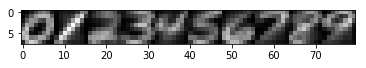
\includegraphics[width=0.5\textwidth]{q2_0_nums.png}
\caption{\label{}Plot of means in each digit class}
\end{figure}



\subsubsection{KNN Euclidean}

\begin{enumerate}[label=(\alph*)]
\item K = 1, test accuracy = 0.96875, train accuracy = 1.0
\item K = 15, test accuract = 0.9585 , train accuracy  = 0.959428571429 
\end{enumerate}

\subsubsection{Break ties}
In my program, I have the array label\char`_count[0 , 10] in function def query\_knn(self, test\_point, k): that stores the number of neighbours with the digit label corresponding to the index of label\_count array. I find the maximum number in label\_count, and the index of the max is the majority vote. If there are multiple, the function label\_count.argmax() will pick the index that comes first. This is justified in class, we can break ties randomly or assign to the first maximum vote.

\subsubsection{K = 1 to 15}



\begin{center}
\begin{tabular}{ |c|c| } 
 \hline
K & Average Fold \\ 
1  &  0.964428571429\\
2  &  0.957571428571\\
3  &  0.963428571429\\
4  &  0.961\\
5  &  0.960857142857\\
6  &  0.959\\
7  &  0.957857142857\\
8  &  0.957428571429\\
9  &  0.955571428571\\
10  &  0.952857142857\\
11  &  0.952285714286\\
12  &  0.951428571429\\
13  &  0.950428571429\\
14  &  0.95\\
15  &  0.948571428571\\
 \hline
\end{tabular}
\end{center}



\begin{center}
\begin{tabular}{ |c|c|c| } 
\hline
K & Training Accuracy & Test Accuracy  \\
1  &  1.0  &  0.96875 \\
2  &  0.982571428571  &  0.96175 \\
3  &  0.983428571429  &  0.96975  \\
4  &  0.978  &  0.9665 \\
5  &  0.977571428571  &  0.96775 \\
6  &  0.974285714286  &  0.9645  \\
7  &  0.973714285714  &  0.96325 \\
8  &  0.970571428571  &  0.9615  \\
9  &  0.969285714286  &  0.9605  \\
10  &  0.967571428571  &  0.961 \\
11  &  0.965428571429  &  0.9595 \\
12  &  0.963142857143  &  0.95825 \\
13  &  0.962428571429  &  0.95775 \\
14  &  0.960142857143  &  0.95775 \\
15  &  0.959428571429  &  0.9585  \\
 \hline
\end{tabular}
\end{center}



%%%%%%%%%%%%%Q 2.2 %%%%%%%%%%%%%%%%%%%
\subsection{Conditional Gaussian}
\subsubsection{Plot of log}
\begin{figure}[H]
\centering
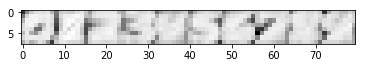
\includegraphics[width=0.5\textwidth]{log_sigma_k.png}
\caption{\label{}log of the diagonal elements of each covariance matrix}
\end{figure}

\subsubsection{average log likelihood}
Train: 40.0734191088 \\
Test: 35.1502166328\\

\subsubsection{Accuracy}
Train 0.981285714286\\
Test 0.95925\\



%%%%%%%%%%%%%%q2.3%%%%%%%%%%%%%%%
\subsection{Naives Bayes}
\subsubsection{Plot of $\eta$}
\begin{figure}[H]
\centering
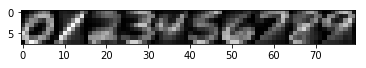
\includegraphics[width=0.5\textwidth]{eta_plot.png}
\caption{\label{}Plot of eta}
\end{figure}


\subsubsection{Plot of new samples}
\begin{figure}[H]
\centering
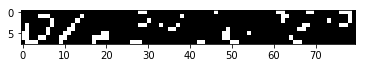
\includegraphics[width=0.5\textwidth]{q3_gen_new.png}
\caption{\label{}Plot of new samples}
\end{figure}

\subsubsection{average log likelihood}
training average log likelihood -30.7898021047\\
testing average log likelihood -30.7369008592
\subsubsection{accuracy}
training accuracy 0.774142857143\\
testing accuracy 0.76425\\

%%%%%%%%%%%%%%Q2.4 %%%%%%%%%%%%
\subsection{summary}
The test accuracy of KNN is 96.875\%, test accuracy of conditional Gaussian is 95.925\%, and Naive Bayes is around 76.425\%. The highest performance is KNN, next followed closely by conditional gaussian, and Naive Bayes is the lowest.\\
This matches my expectation because KNN is inferring class label based on neighbours, and conditional Gaussian is using shared covariance matrix. Our data set, handwritten digits, have very similar form in one class. In both KNN and conditional Gaussian, we are assuming that images in each class are similar, and we predict based on what we have seen already in a class.\\
In Naive Bayes, however, we assume that all data are independent from each other. This assumption unfortunately does not hold in this dataset, and therefore reducing accuracy of our predictions.


% \section{Some examples to get started}

% \subsection{How to add Comments}

% Comments can be added to your project by clicking on the comment icon in the toolbar above. % * <john.hammersley@gmail.com> 2014-09-03T09:54:16.211Z:
% %
% % Here's an example comment!
% %
% To reply to a comment, simply click the reply button in the lower right corner of the comment, and you can close them when you're done.

% \subsection{How to include Figures}

% First you have to upload the image file from your computer using the upload link the project menu. Then use the includegraphics command to include it in your document. Use the figure environment and the caption command to add a number and a caption to your figure. See the code for Figure \ref{fig:frog} in this section for an example.

% \begin{figure}
% \centering
% \includegraphics[width=0.3\textwidth]{frog.jpg}
% \caption{\label{fig:frog}This frog was uploaded via the project menu.}
% \end{figure}

% \subsection{How to add Tables}

% Use the table and tabular commands for basic tables --- see Table~\ref{tab:widgets}, for example. 


% \subsection{How to write Mathematics}

% \LaTeX{} is great at typesetting mathematics. Let $X_1, X_2, \ldots, X_n$ be a sequence of independent and identically distributed random variables with $\text{E}[X_i] = \mu$ and $\text{Var}[X_i] = \sigma^2 < \infty$, and let
% \[S_n = \frac{X_1 + X_2 + \cdots + X_n}{n}
%       = \frac{1}{n}\sum_{i}^{n} X_i\]
% denote their mean. Then as $n$ approaches infinity, the random variables $\sqrt{n}(S_n - \mu)$ converge in distribution to a normal $\mathcal{N}(0, \sigma^2)$.


% \subsection{How to create Sections and Subsections}

% Use section and subsections to organize your document. Simply use the section and subsection buttons in the toolbar to create them, and we'll handle all the formatting and numbering automatically.

% \subsection{How to add Lists}

% You can make lists with automatic numbering \dots

% \begin{enumerate}
% \item Like this,
% \item and like this.
% \end{enumerate}
% \dots or bullet points \dots
% \begin{itemize}
% \item Like this,
% \item and like this.
% \end{itemize}

% \subsection{How to add Citations and a References List}

% You can upload a \verb|.bib| file containing your BibTeX entries, created with JabRef; or import your \href{https://www.overleaf.com/blog/184}{Mendeley}, CiteULike or Zotero library as a \verb|.bib| file. You can then cite entries from it, like this: \cite{greenwade93}. Just remember to specify a bibliography style, as well as the filename of the \verb|.bib|.

% You can find a \href{https://www.overleaf.com/help/97-how-to-include-a-bibliography-using-bibtex}{video tutorial here} to learn more about BibTeX.

% We hope you find Overleaf useful, and please let us know if you have any feedback using the help menu above --- or use the contact form at \url{https://www.overleaf.com/contact}!

% \bibliographystyle{alpha}
% \bibliography{sample}

\end{document}